% ---- Top row: bullets + Chooz uncertainty plot, side by side ----
\begin{minipage}[t]{0.56\linewidth}
\begin{itemize}
    \item Conventional uncertainty calculation:
    \begin{equation}
      \boxed{\Delta \varphi = \arctan \left( \frac{P/l}{\sqrt N} \right)}
      \label{eq:deltaphi}
    \end{equation}
    \item If mean position resolution \(P\rightarrow0\), angular uncertainty \(\Delta\varphi\rightarrow0\) -- unphysical!
    \item Vogel and Beacom model shows a large spread (\(\sim26^\circ\)) in intial neutron direction
    \item Neutrons scatter many times before capture
\end{itemize}
\end{minipage}
\hfill
\begin{minipage}[t]{0.40\linewidth}
    \vspace{0pt}
    \centering
    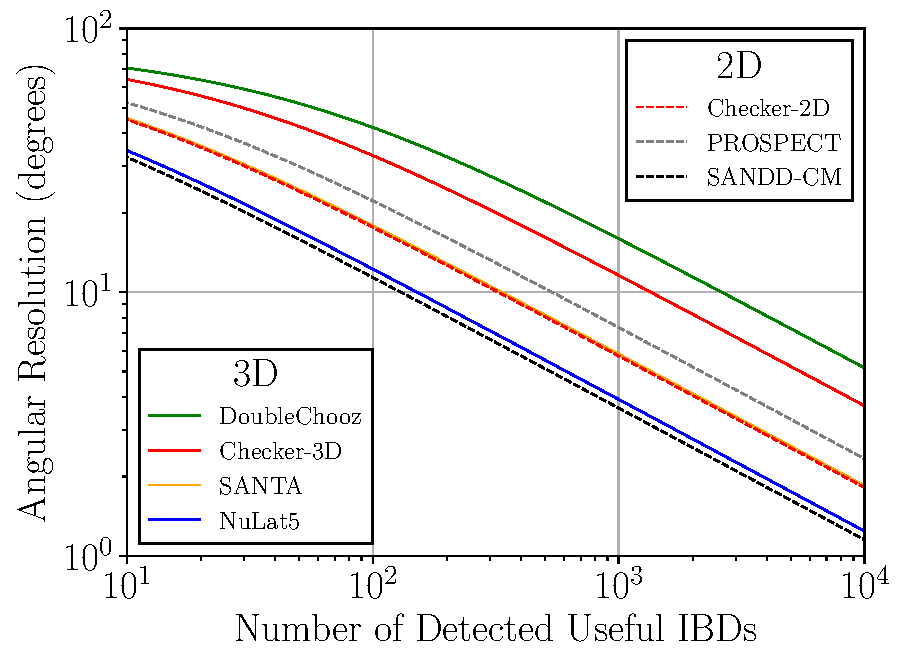
\includegraphics[width=\linewidth]{fig/angular_resolution_analytic_ylog_PackFactor_v2Useful.pdf}
    \captionof{figure}{Angular uncertainty calculated using the conventional ``Chooz'' approach, used in our previous study~[2].}
    \label{fig_old_method}
\end{minipage}

\vspace{0.5cm}

% ---- Additional content from Paper A: psi-geometry diagram, full width, scaled to fit ----
\begin{center}
\setlength{\unitlength}{.1\linewidth}
\resizebox{0.62\linewidth}{!}{%
\begin{picture}(10,4)
  \put(10,3){\color{gray}\line(-1,0){4}} % neutrino
  \put(10,3){\vector(-1,0){1.5}} % neutrino

  \put(1,3){\vector(1,0){1}} % x axis
  \put(1,3){\vector(0,1){1}} % y axis
  \put(1,3){\vector(-1,-2){.3}} % z axis
  \put(1.75, 2.65){$x$}
  \put(0.65, 3.65){$y$}
  \put(0.45, 2.45){$z$}

  \put(6,3){\color{black}\circle*{.25}} % IBD vertex
  \put(6.5,1.5){\color{black}\circle*{.25}} % e+ annihilation
  \put(1,.5){\color{black}\circle*{.25}} % n capture

  \put(6,3){\vector(-1,-0.2){1}} % neutron
  \put(6,3){\vector(.5,-1.5){.25}} % e+
  \put(6,3){\line(.5,-1.5){.5}} % e+
  % text:
  \put(5.7, 3.5){\text{IBD}}
  \put(5., 3.){\text{n}}
  \put(8.6, 3.5){$\bar\nu_e$}
  \put(6.4,2.4){\text{e}$^+$}
  \put(7.,1.3){\text{e}$^+$ \text{annihilation}}
  \put(0,0){\text{neutron capture}}

  % direction vectors:
  \put(1,.5){\vector(1,0){4}} % S_T
  \put(1,.5){\color{gray}\line(6.5,1.9){5.3}} % gray line along S_R
  \put(1,.5){\vector(6.5,1.9){3.5}} % S_R
  % text:
  \put(4.7,0){$S_T$}
  \put(3.7,1.8){$S_R$}

% THE MAIN ANGLE PSI:
  \put(2.7,0.7){\texttt{$\psi$}}
  \put(1,.5){\arc[0,16.5]{1.55}} % angle phi_nu
  \put(1,.5){\arc[0,16.5]{1.5}} % angle phi_nu
\end{picture}%
}
\end{center}
\captionof{figure}{Definition of the reconstruction angle $\psi$ between the true source direction $S_T$ and the reconstructed direction $S_R$ (neutron-capture vertex $\rightarrow$ positron-annihilation vertex). The antineutrino source lies along $x$; $\psi = 0$ is perfect reconstruction.}
\label{fig:recon}
% --- Original (full) caption, kept for reference / restore: ---
% Diagram of how the angle $\psi$ between reconstructed $S_R$ and true $S_T$ source direction is defined.
% The vector $S_R$ points from the reconstructed vertex of the neutron capture towards the reconstructed vertex where positron deposited its energy before annihilating. The MeV-scale positron travels a few millimeters before being annihilated with an electron.
% The keV-scale neutron loses its energy in the detector medium before being captured; the separation between IBD vertex and the capture location could be made large if there is no medium in between, as in some of the detector designs considered in this study.
% The antineutrino source was positioned along the $x$-axis: angle $\psi = 0$ would indicate a perfect reconstruction of direction.
